\chapter{Testy}\label{cha:pierwszyDokument}

Ogolnie :
zlozonosc algorytmu, zajmowana pamiec

Poszczegolnych:
szybkosc funkcji, odchylenie standardowe , srednie itp z np 20 runów, runy zrobic tez dla roznych ilosci iteracji bo moze sie cos nie wyrabia i potem jest lepiej 
%---------------------------------------------------------------------------

\section{Metody selekcji}\label{sec:strukturaDokumentu}

Analiza metod selekcji w obrębie jednej instancji została przeprowadzona przy założeniu stałych takich jak:
\begin{itemize}
\item
 warunki początkowe, a więc stałej macierzy odległości, macierzy przepływu,
\item
początkowa populacja,
\item
metoda selekcji,
\item
metoda krzyżowania,
\item
ilość iteracji algorytmu
\end{itemize}
\par
\vspace{0,4cm}
Testy zostały przeprowadzone dla poniżej zaprezentowanych instancji danych wejściowych, zaczerpniętych z WSTAWIĆ BIBLIOGRAFIUE, gdzie również znajduje się informacja o najlepszym otrzymanym wyniku funkcji celu dla danej instancji danych. Dzięki temu możliwe jest określenie jak blisko rozwiązania znajduje się wynik działania algorytmu dla każdej z metod. W celu uzyskania ostatecznego rozwiązania, a więc rozwiązania nie zmieniającego się dalej pod wpływem kolejnych iteracji algorytmu, analiza została przeprowadzona dla odpowiednio 20 000 oraz 50 000 iteracji.\\

\subsection{Dane wejściowe instancja I}

\par
$$
\mathbf{Macierz\_przepływu} =
\left( \begin{array}{cccccccccccc}
0& 1& 2& 2& 3& 4& 4& 5& 3& 5& 6& 7\\
1& 0& 1& 1& 2& 3& 3& 4& 2& 4& 5& 6\\
2& 1& 0& 2& 1& 2& 2& 3& 1& 3& 4& 5\\
2& 1& 2& 0&1& 2& 2& 3& 3& 3& 4& 5\\
3& 2& 1& 1& 0& 1& 1& 2& 2& 2& 3& 4\\
4& 3& 2& 2& 1& 0& 2& 3& 3& 1& 2& 3\\
4& 3& 2& 2& 1& 2& 0& 1& 3& 1& 2 & 3\\
5& 4& 3& 3& 2& 3& 1& 0& 4& 2& 1& 2\\
3& 2& 1& 3& 2& 3& 3& 4& 0& 4& 5& 6\\
5& 4& 3& 3& 2& 1& 1& 2& 4& 0& 1& 2\\
6& 5& 4&4& 3& 2& 2& 1& 5& 1& 0& 1\\
7& 6& 5& 5& 4& 3& 3& 2& 6& 2& 1& 0 \\
\end{array} \right)
$$

\par
$$
\mathbf{Macierz\_odległości} =
\left( \begin{array}{cccccccccccc}
0&3&4&6&8&5&6&6&5&1&4&6\\
3&0&6&3&7&9&9&2&2&7&4&7\\
4&6&0&2&6&4&4&4&2&6&3&6\\
6&3&2&0&5&5&3&3&9&4&3&6\\
8&7&6&5&0&4&3&4&5&7&6&7\\
5&9&4&5&4&0&8&5&5&5&7&5\\
6&9&4&3&3&8&0&6&8&4&6&7\\
6&2&4&3&4&5&6&0&1&5&5&3\\
5&2&2&9&5&5&8&1&0&4&5&2\\
1&7&6&4&7&5&4&5&4&0&7&7\\
4&4&3&3&6&7&6&5&5&7&0&9\\
6&7&6&6&7&5&7&3&2&7&9&0\\
\end{array} \right)
$$

\par
$$
\mathbf{Pierwsza\_populacja} =
\left( \begin{array}{cccccccccccc}
6&1&9&2&7&3&10&8&4&11&5&12\\
4&3&9&7&5&12&8&2&11&10&1&6\\
11&7&10&6&8&9&12&5&2&1&3&4\\
3&11&2&5&4&7&10&8&12&6&9&1\\
8&4&10&7&5&3&12&9&6&1&2&11\\
2&12&10&3&6&7&1&11&4&5&8&9\\
9&4&2&7&3&12&8&11&1&5&10&6\\
2&5&7&12&6&8&9&11&4&1&3&10\\
6&7&1&4&11&9&8&3&2&5&12&10\\
3&6&7&9&10&1&12&11&8&4&2&5\\
2&11&8&6&9&4&10&5&1&12&3&7\\
12&3&5&4&9&8&6&11&2&7&10&1\\
\end{array} \right)
$$


\begin{itemize}
\item  \textbf{20 000 iteracji}\\
\par
 MOZNA DODAC JESCZE PORÓWNANIE SZYBKOSCI DZIAŁANIA POSZCZEGOLNYCH METOD
 W \ref{instancja_1} zostały zestawione wartości funkcji celu w kolejnych iteracjach dla poszczególnych metod selekcji. Metody selekcji zostały szczegółowo opisane w \ref{metody_selekcji}. Dla każdej z metod została policzona średnia wartość funkcji celu, odchylenie standardowe oraz współczynnik zmienności będący stosunkiem wartości odchelenia standardowego i średniej. Za pomocą tych narzędzi statystycznych można określić zachowanie poszczególnych metod oraz wyodrębnić metodę dającą w tym kontekście najbardziej satysfakcjonujący wynik. Kolorem zielonym został również zaznaczony najlepszy otrzymany wynik.\\
\par
\begin{table}[h!]
\begin{center}
\scalebox{0.6}{
\begin{tabular}{|c|c|c|c|c|c|c|c|c|}
\hline
\textbf{Iteracja}  &\textbf{Losowa}  & \textbf{Rankingowa} & \textbf{Ruletka} & \textbf{Turniejowa} & \textbf{Elitarna} & \textbf{Losowa 2} & \textbf{Rankingowa 2} & \textbf{Turniejowa 2}\\
\hline
 \textbf{1}&1676&1662&1700&1666&1686&1688&1668	&1760 \\
\hline
 \textbf{2}&1680&1662&1664&1666&1676&1682&1682&1756 \\
\hline
 \textbf{3}&1668&1664&1710&1672&1680&1682&1672&1796  \\
\hline
 \textbf{4}&1666&1664&1694&1696&1682&1680&1702	&1742  \\
\hline
 \textbf{5}&1666&1672&1692&1706&1692&1672&1672&1820  \\
\hline
 \textbf{6}&1670&1660&1706&1680&1670&1682&1670&1798\\
\hline
 \textbf{7}&1666&1666&1708&1690&1670&1680&1702&1766 \\
\hline
 \textbf{8}&1670&1656&1722&1676&1668&1688&1686	&1700\\
\hline
 \textbf{9}&1692&1666&1662&1656&1680&1708&1678	&1706\\
\hline
 \textbf{10}&1668&1656&1670&1676&1674&1716&1706&1826\\
\hline
 \textbf{11}&1682&1660&1688&1670&1690&1712&1682&1778 \\
\hline
 \textbf{12}&1696&1660&1716&1688&1678&1728&1660&1770 \\
\hline
 \textbf{13}&1668&\color{green}\textbf{1654}&1692&1688&1684&1702&1672&1774 \\
\hline
 \textbf{14}&1668&1660&1668&1672&1706&1696&1698&1728\\
\hline
 \textbf{15}&1696&1664&1672&1688&1684&1684&1684&1806\\
\hline
 \textbf{16}&1714&1660&1686&1676&1674&1676&1690&1774\\
\hline
 \textbf{17}&1662&1656&1700&1674&1676&1684&1684&1758 \\
\hline
 \textbf{18}&1678&1662&1672&1672&1690&1692&1680&1746\\
\hline
 \textbf{19}&1670&1666&1718&1680&1680&1712&1662&1762\\
\hline
 \textbf{20}&1684&1660&1682&1666&1674&1666&1670&1720\\
\hline
 \textbf{ŚREDNIA}&1677&1661&1691&1677&1680&1691&1681&1746\\
\hline
 \textbf{ODCHYLENIE STANDARDOWE}&13,15&4,19&18,35&11,56&8,86&16&13,02&33,9\\
\hline
 \textbf{WSPÓŁCZYNNIK ZMIENNOŚCI}&0,78\%&0,25\%&1,09\%&0,69\%&0,53\%&0,95	\%&0,77\%&1,92\%\\
\hline
\end{tabular}}
\caption{Wartości funkcji celu dla poszczególnych metod selekcji}
\label{instancja1}
\end{center}
\end{table}


Na podstawie powyższej tabeli zauważalny staje się fakt iż najbardziej satysfakcjonujące wyniki w przeciągu 20 000 iteracji otrzymuje metoda rankingowa. W 15 na 20 przypadków uzyskała ona najmniejsze wartości funkcji celu. W pozostałych przypadkach znajduje się na drugim bądź też trzecim miejscu. Posiada ona również najmniejszy współczynnik odchylenia standardowego oraz współczynnik zmienności co świadczy o stosunkowo najbliższym spośród wszystkich metod położeniu wyników wokół wartości średniej. Poniżej zestawiony został ranking metod selekcji utworzony w zależności od uzyskanej wartości średniej funkcji celu.\\



\begin{table}[h!]
\begin{center}
\scalebox{0.8}{
\begin{tabular}{|c|c|c|}
\hline
\textbf{Miejsce}  &\textbf{Metoda}  & \textbf{Funkcja celu}\\
\hline
 \textbf{1}&Rankingowa&1661 \\
\hline
 \textbf{2}&Turniejowa&1677\\
\hline
 \textbf{3}&Losowa&1677\\
\hline
 \textbf{4}&Elitarna&1680\\
\hline
 \textbf{5}&Rankingowa 2&1681\\
\hline
 \textbf{6}&Ruletki&1691\\
\hline
 \textbf{7}&Losowa 2&1691\\
\hline
 \textbf{8}&Turniejowa 2&1746\\
\hline
\end{tabular}}
\caption{Ranking metod selekcji na podstawie średniej wartości funkcji celu}
\label{ranking_1}
\end{center}
\end{table}

Widoczny staje się więc fakt iż lepiej działają metody w których stosujemy ograniczenia co do konieczności nie powtarzania się danego rodzica w grupie rodzicielskiej. A więc metody Rankingowa, Losowa oraz Turniejowa. Nie mniej jednak w gronie metod nie stosujących się do zasady indywidualności osobnika najwyższe miejsce w rankingu otrzymuje również metoda Rankingowa. Przebieg działania algorytmu dla poszczególnych metod można przenalizować na podstawie poniższego wykresu. Na wykresie tym został zaprezentowany przebieg dla którego to wartość końcowa uzyskana przez metode rankingową jest jednocześnie najmniejszą wartością funkcji celu otrzymaną w we wszystkich 20 iteracjach.\\
\begin{figure}[ht]
		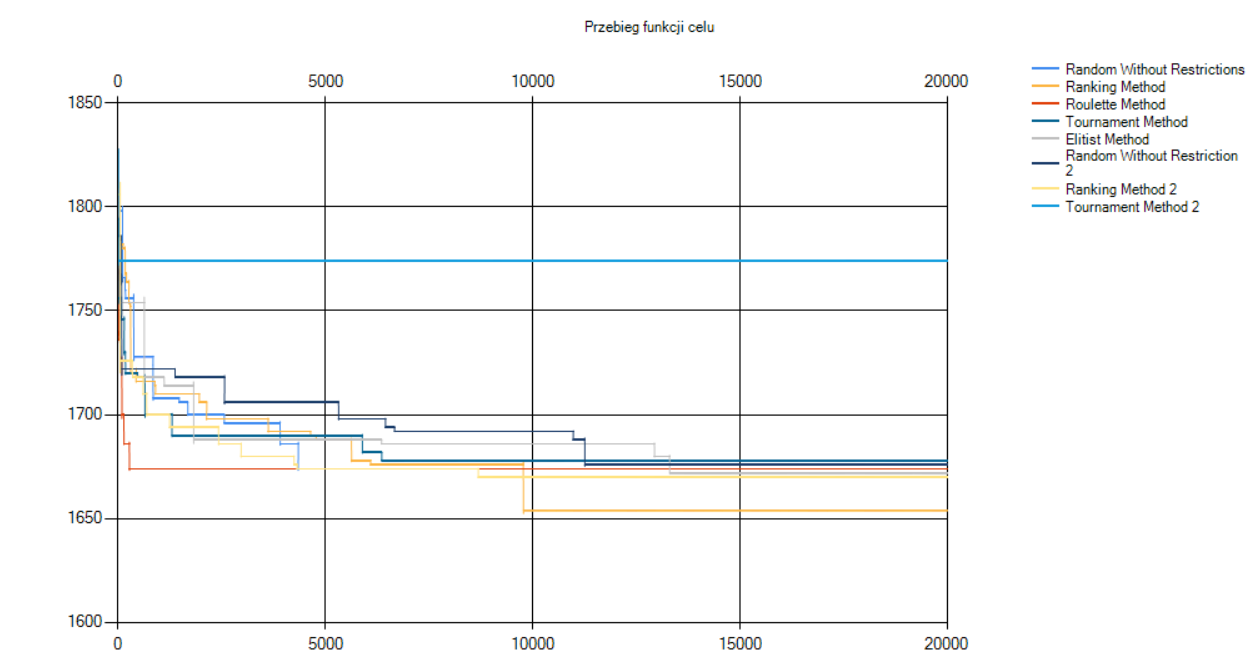
\includegraphics[scale=0.6]{../../../../../Screeny/matody_1654_legend.png}
		\caption{Przebiej działania algorytmu dla poszczególnych metod selekcji}
		\label{ranking}			
\end{figure}

Na podstawie \ref{ranking_1} zauważalne staje się zmniejszanie się wartości funkcji celu w kolejnych iteracjach algorytmu.  W przypadku metod takich jak metoda ruletki czy też metoda turniejowa, która dopuszcza powtórzeń wśrod osobników w grupie rodzicielskiej, stabilizacja poziomu następuje w początkowych iteracjach i utrzymuje się tak do końca. Powodem tak szybkiej zbieżności tych metod jest brak różnorodności w kolejnych grupach rodzicielskich. W metodzie ruletki spowodowane jest to dużym prawdopodobieństwem wylosowania osobnika najlepszego co prowadzi do jego dominanty nad innymi. Natomiast w metodzie selekcji turniejowej turniej jest w większości przypadków wygrywany przez ten sam osobnik, co przy dodatkowym założeniu iż w jednej grupie rodzicielskiej mogą znajdować się te same osobniki prowadzi do sytuacji że na grupę rodzicielską składają się 3 te same osobniki. Pomimo wrażenia iż rozwiązania osiągnęły stan stabilny już w 20 000 itreracji, należy sprawdzić czy nie nastąpi jeszcze spadek wartości funkcji celu gdy liczba iteracji zostanie zwiększona. W tym celu ponowione zostają badania metod dla 50 000 iteracji.\\

\item  \textbf{50 000 iteracji}
\end{itemize}



WNIOSKI
- W ilu iteracjch wygrywała jednak rnkingowa w 17 na 20
- 20 000 operacji najlepszy wynik to 1654
-raczej 20 000 operacji jest wystarczajace ale nie zawsze sie wyrabia
- ruletki działa słabo, jest jedn pik w dół i potem juz prawie zawsze do końca jest na tym samym poziomie ( mozna dac wykres przykładowo oprazujący o co chodzi)
-jak w stosunku do powtarzajacych się działaja te nie powtrzajace sie

\subsection{Dane wejściowe instancja II}